\documentclass{standalone}

\usepackage{standalone}
\usepackage{tikz}
\usetikzlibrary{calc,intersections}

\begin{document}
	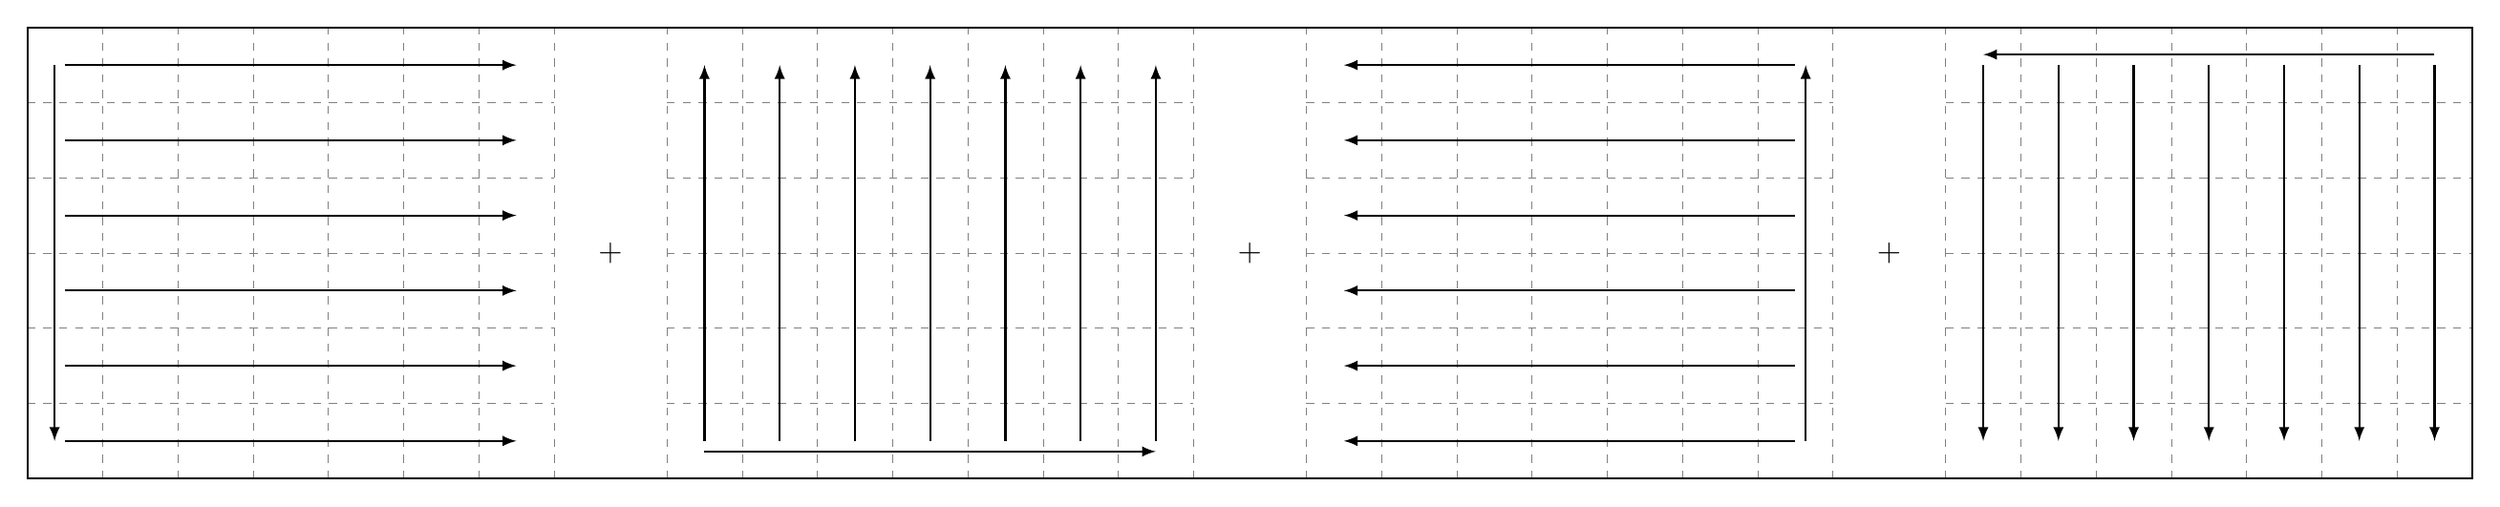
\begin{tikzpicture}
	
		\pgfmathtruncatemacro{\xsize}{7}
		\pgfmathtruncatemacro{\ysize}{6}


		\pgfmathsetmacro{\arrowoffset}{0.07}
		\pgfmathsetmacro{\intergriddistance}{1.5}
		
		% draw 4 grids
		\foreach \ngrid in {0, ..., 3}
		{
			\begin{scope}[shift={(\ngrid * \xsize + \ngrid * \intergriddistance, 0)}]
				\draw[dashed, very thin, black!50] (0,0) grid (\xsize, \ysize);
			\end{scope}
		}		
	
		\draw[thick]
			(0, 0) --
			++ (0, \ysize) --
			++ (4 * \xsize + 3 * \intergriddistance, 0) --
			++ (0, -\ysize) --
			cycle;

		\pgfmathtruncatemacro{\xinnersize}{\xsize - 1}
		\pgfmathtruncatemacro{\yinnersize}{\ysize - 1}
		
		% draw +s
		\foreach \i in {1, 2, 3}
		{
			\node at (\i * \xsize + \i * \intergriddistance - \intergriddistance / 2, \ysize / 2) {\large + };
		}
		
		% draw first run
		\begin{scope}[shift={(0.5, -0.5)}, thick]
			\foreach \row in {1, ..., \ysize}
			{
				\draw[-latex] (0, \row) -- ++(\xinnersize, 0); % arrow right
			}
			\draw[-latex] (0 - 2 * \arrowoffset, \ysize) -- ++(0, -\ysize + 1); % arrow down
		\end{scope}
		
		% draw second run
		\begin{scope}[shift={(1 * \xsize + 1 * \intergriddistance, 0)}]
			\begin{scope}[shift={(-0.5, 0.5)}, thick]
				\foreach \col in {1, ..., \xsize}
				{
					\draw[-latex] (\col, 0) -- ++(0, \yinnersize); % arrow up
				}
				\draw[-latex] (1, 0 - 2 * \arrowoffset) -- ++(\xsize - 1, 0); % arrow right
			\end{scope}
		\end{scope}
		
		% draw third run
		\begin{scope}[shift={(2 * \xsize + 2 * \intergriddistance, 0)}]
			\begin{scope}[shift={(0.5, -0.5)}, thick]
				\foreach \row in {1, ..., \ysize}
				{
					\draw[-latex] (\xinnersize, \row) -- ++(-\xinnersize, 0); % arrow left
				}
				\draw[-latex] (\xsize - 1 + 2 * \arrowoffset, 1) -- ++(0, \ysize - 1); % arrow up
			\end{scope}
		\end{scope}
		
		% draw forth run
		\begin{scope}[shift={(3 * \xsize + 3 * \intergriddistance, 0)}]
			\begin{scope}[shift={(-0.5, 0.5)}, thick]
				\foreach \col in {1, ..., \xsize}
				{
					\draw[-latex] (\col, \yinnersize) -- ++(0, -\yinnersize); % arrow down
				}
				\draw[-latex] (\xsize, \yinnersize + 2 * \arrowoffset) -- ++(-\xsize + 1, 0); % arrow left
			\end{scope}
		\end{scope}
		
	\end{tikzpicture}
\end{document}
